\section{Discussion}

\subsection{Justification of DeepGeo's Over-Parameterization and Complexity}
\label{ch5:sec:complexity}

Traditional parameterizations rely on low-dimensional design variables and suffer from several key limitations:
\begin{itemize}
    \item They require extensive manual intervention. This includes selecting an appropriate method, configuring parameters to balance flexibility, smoothness and robustness, and carefully defining parameter constraints. Moreover, capturing essential inter-parameter correlations--such as the twisting or sweeping global functions used in wing optimization--must be explicitly hard-coded, which heavily depends on domain expertise.

    \item They rely on costly trial-and-error procedures. The quality of results often depends on iterative manual experimentation. For example, an inappropriate FFD configuration of a CRM wing can lead to a 42\% reduction in drag improvement~\cite{aa.Lyu2015}, making multiple optimization attempts necessary to achieve a near-optimal design.
\end{itemize}

In contrast, DeepGeo leverages over-parameterization to enable its capability, adaptability and robustness. The large number of parameters is not a drawback but a necessary design choice that allows DeepGeo to capture complex geometric variations and to implement the benefits described above through a fully automatic, data-independent process. During its initialization phase, as defined by Eq.~\ref{ch5:eq:weightInit}, DeepGeo automatically learns a design parameterization by combining the selection, setting and integration of parameters into an adaptive framework. Consequently, DeepGeo’s most significant advantages over traditional parameterizations are the reduction in manual intervention, minimized dependency on expert prior and the elimination of costly trial-and-error practices.

% !TEX root = ../main.tex
% !TEX spellcheck = en-US

\begin{figure}[tbh]
    \begin{center}
        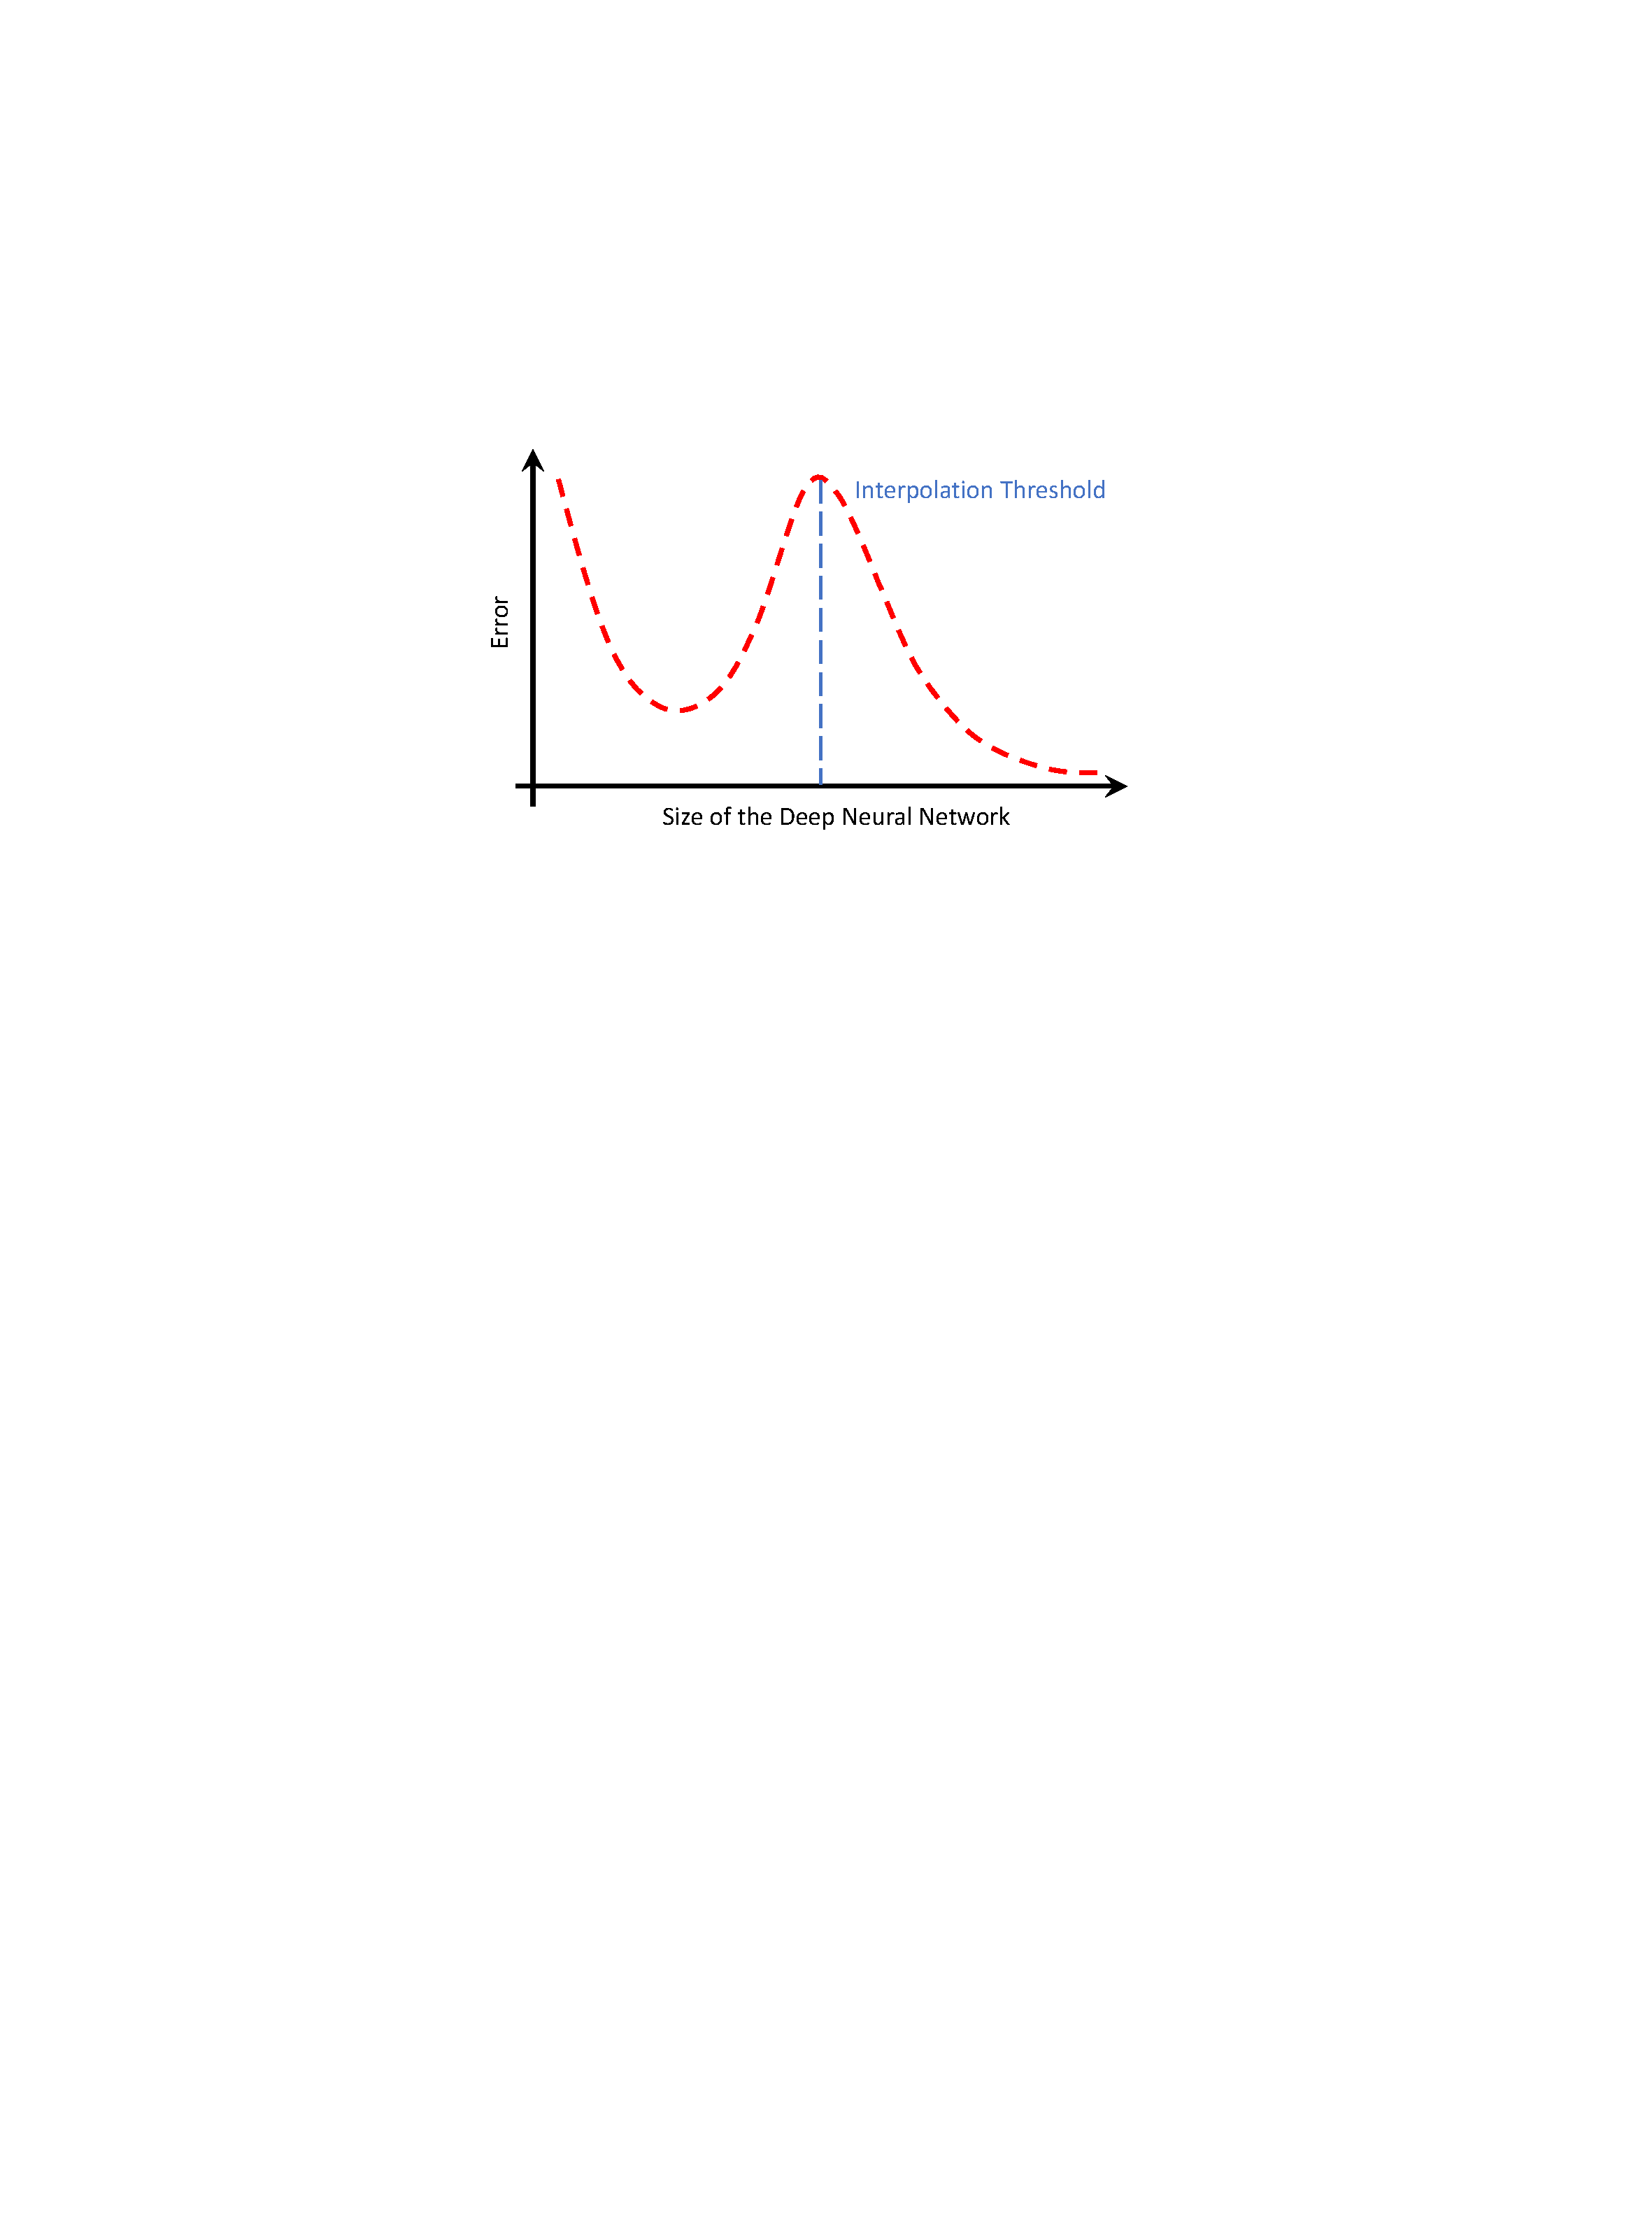
\includegraphics[width=1\linewidth]{chapter5/fig/double_descent.pdf}
    \end{center}
    \vspace{-5mm}
    \caption{
        \small  The \textit{double descent} phenomenon in deep learning models.
    }
    \label{ch5:fig:double_descent}
\end{figure}

Using the number of weights for as a proxy for  DeepGeo's actual complexity is misleading when comparing it to methods that do not rely on deep learning. This is because in DeepGeo, as in most deep-learning approaches with high-dimensional parameter spaces,
the large parameter count does not necessarily translate into excessive complexity. Recent studies have revealed the \textit{double descent} phenomenon~\cite{ai.Belkin2019,ai.Spigler2019}, as illustrated in Fig.~\ref{ch5:fig:double_descent}, which shows that as model size increases, the generalization error first decreases, then rises near the interpolation threshold, and finally decreases again with further over-parameterization. This second descent implies that highly over-parameterized models can be more effective despite their excessive parameter amount. This behavior is due to the weight correlations developed in neural networks~\cite{ai.Jin2020b} and the reduced number of independent degrees of freedom during training. Therefore, a more meaningful indicator of DeepGeo's complexity is its \textit{effective dimensionality}, which quantifies the number of independent directions in parameter space that influence the model’s behavior--akin to reduced dimensions in model order reduction. A well-trained network typically exhibits low \textit{effective dimensionality}, meaning that its function lies in a relatively low-dimensional parameter subspace despite its large number of parameters, and it can effectively compress the information from data.
\begin{table}[htbp]
  \centering
  \caption{Comparison of effective dimensionality for DeepGeo models. The values of random model are based on 20 repeats.}
  \resizebox{\textwidth}{!}{  
    \begin{tabular}{llllll}
    \hline
    \multirow{2}[2]{*}{\textbf{Model}} & \textbf{Layer 1} & \textbf{Layer 2} & \textbf{Layer 3} & \textbf{Output Layer} & \multirow{2}[2]{*}{\textbf{Overall}}\\
           & weight ratio: $0.1\%$ & weight ratio: 11.0\% & weight ratio: 87.9\% & weight ratio: 1.0\% &  \\
    \hline
    Random & $264.0\pm44.9$ & $114.4\pm63.1$ & $226.5\pm33.5$ & $332.7\pm34.4$ & $215.3\pm37.1$ \\
    \hline
    2D Circle & $2.6$  & $2.9$  & $2.6$  & $3.9$  & $2.6$ \\
    \hline
    CRM Wing & $2.3$  & $0.4$  & $0.1$  & $4.8$  & $0.2$ \\
    \hline
    BWB Aircraft & $134.8$ & $51.5$ & $24.6$ & $-0.5$ & $27.4$ \\
    \hline
    \end{tabular}%
  }
  \label{ch5:tab:double_descent}%
\end{table}%

To empirically validate this, we compute DeepGeo’s \textit{effective dimensionality} using a metric based on the eigenvalues of the symmetric Hessian matrix of DeepGeo's weights~\cite{ai.Maddox2020} (as defined by Equation~\ref{ch5:eq:response_effective_dimensionality}). More details are included in Appendix~\ref{ch5:sec:appendix_effe_dim}. As shown in Table~\ref{ch5:tab:double_descent}, the initialized DeepGeo model has significantly lower effective dimensionalities compared to randomly initialized ones. This supports our claim that DeepGeo’s actual complexity is far less than its parameter count may suggest.

\subsection{Justification of DeepGeo's Smoothness, Expressiveness and the Role of $L_{reg}$}

DeepGeo provides both global surface smoothness and sufficient deformation freedom to support high-fidelity design optimization. Several factors contribute to this. First, the smoothness arises naturally from the inherent properties of its MLP backbone, known in literature as the frequency principle~\cite{ai.Xu2019f,ai.Xu2020c} or spectral bias~\cite{ai.Rahaman2019}. As a result, the network tends to prioritize low-frequency features, while high-frequency components typically require more training iterations to emerge. Since ASO usually requires fewer iterations to converge than for  typical deep learning training, undesired high-frequency patterns, such as bumps or discontinuities, are unlikely to appear. Second, DeepGeo learns to create a shape deformation field rather than a full geometry from scratch and such a field is inherently smoother. For instance, when deforming an airfoil, DeepGeo does not need to reconstruct sharp trailing edges or rounded leading edges from zero. Instead, it learns a smooth transformation that modifies these features, simplifying the learning and contributing to overall surface regularity. Third, the use of a gradient-descent-based optimizer leads to smooth transitions in the design trajectory. At each iteration, the newly deformed geometry is a slight variant of the previous one. This mostly avoids abrupt or unstable geometric transformations.

DeepGeo’s expressiveness is supported by its over-parameterized MLP structure and, according to the universal approximation theory~\cite{ai.Barron1993,ai.Poggio2017}, this expressiveness is up-bounded by the model size. However, empirical results in Section~\ref{ch5:sec:complexity} show that the current model size has enabled the over-parameterization effect for all ASO tasks presented in this work. If DeepGeo were to be applied to significantly more complex tasks, increasing model size might be necessary.

The Hessian-based regularization loss $L_{reg}$, though introduced to stabilize volumetric mesh deformation, directly penalizes the magnitude of the network’s Hessian, and could potentially constrain DeepGeo's frequency behavior. While a full understanding of theoretical effects of this regularization on the model’s spectral properties would require further investigation, our empirical results do not indicate a significant loss in DeepGeo's expressiveness when $L_{reg}$ is properly weighted. As shown in Figure~\ref{ch5:fig:w_loss_reg_ablation}, even changing the weight of $L_{reg}$ by several orders of magnitude produces nearly identical deformed shapes. Furthermore, we analyze the gradient magnitudes of $\cO_{CFD}$ and $L_{reg}$ with respect to DeepGeo’s parameters at the start of design optimization. As shown in Table~\ref{ch5:tab:gradient_norm}, the norm of $\nabla L_{reg}$ is multiple orders of magnitude smaller than that of $\nabla \cO_{CFD}$ across all layers. This demonstrates that the physical objective driven by the adjoint solver is the dominant force that shapes DeepGeo's behavior.

\begin{table}[htbp]
  \centering
  \caption{The comparison of mean vector norms of $\nabla \cO_{CFD}$ and $\nabla L_{reg}$ with respect to all DeepGeo's layers}
    \begin{tabular}{lcccc}
    \hline
    \multirow{2}[4]{*}{ASO Case} & \multicolumn{4}{c}{Mean Vector Norm of $\nabla \cO_{CFD}$}\\
\cline{2-5}           & Layer 1 & Layer 2 & Layer 3 & Output Layer\\
    \hline
    2D Circle & 0.1825 & 0.4186 & 0.5105 & 6.3915\\
    CRM Wing & 0.1254 & 0.2814 & 0.2411 & 6.4747 \\
    BWB Aircraft & 0.1137 & 0.2166 & 0.1495 & 1.3316\\
    \hline
    \multirow{2}[4]{*}{ASO Case} & \multicolumn{4}{c}{Mean Vector Norm of $\nabla L_{reg}$}\\
\cline{2-5}           & Layer 1 & Layer 2 & Layer 3 & Output Layer\\
    \hline
    2D Circle & 0.0003 & 0.0003 & 0.0009 & 0.0235\\
    CRM Wing & 9.4266$\times 10^{-5}$ & 9.9453$\times 10^{-5}$ & 3.8320$\times 10^{-5}$ & 0.0016 \\
    BWB Aircraft & 0.0009 & 0.0008 & 0.0003 & 0.0034\\
    \hline
    \end{tabular}%
  \label{ch5:tab:gradient_norm}%
\end{table}%

Additionally, DeepGeo is different from traditional spectral parameterization methods used in ASO, such as \citet{aa.Li2019c,aa.Li2021c}. Those methods rely on explicit mode truncation for dimensionality reduction, which limits the design space in advance. In contrast, DeepGeo does not manually cut off its spectrum, it instead adapts its behavior according to different geometries and design tasks through its optimization.

Recent advances in computer vision and graphics have introduced techniques such as positional embeddings~\cite{ai.Vaswani2017} and feature grids~\cite{ai.Mueller2022} to inject high-frequency detail into MLPs. These techniques offer promising directions for future work aimed at implementing DeepGeo’s controllable smoothness and expanding the model's expressiveness when needed.

\section{Conclusion}
This research introduces a novel framework that leverages deep geometric learning to implement a fully automated shape parameterization method for Aerodynamic Shape Optimization (ASO).
By automating the parameterization process, DeepGeo significantly enhances efficiency and robustness over traditional methods, minimizing the need for manual intervention while maintaining optimization performance that is either superior or at least comparable to the best manually tuned techniques.
Specifically, in comparison to the state-of-the-art Free-Form Deformation (FFD) model, DeepGeo fully automates the handling of diverse geometries in both 2D and 3D. In contrast, FFD requires users to design a custom configuration for each task to achieve optimal performance, which demands extensive tuning and strong domain prior knowledge.

Additionally, DeepGeo integrates Computational Fluid Dynamics (CFD) mesh deformation directly into the parameterization model within the adjoint-based ASO pipeline, whereas traditional methods rely on a separate module to address meshing issues as pre-processing to physical simulations
This integration simplifies the ASO pipeline and removes the need for additional mesh management.
Furthermore, DeepGeo offers significant freedom in shape deformation while maintaining global surface smoothness. For example, in the case study that optimizes a 2D circle, DeepGeo successfully converges to a solution without complex adjustments, whereas FFD encounters substantial challenges and fails to achieve convergence. The necessary remedy for FFD were complex and non-trivial~\cite{aa.He2019}.
Notably, DeepGeo works without requiring any training data, while it still leverages the strengths of deep learning to manage high-dimensional optimization problems.
This data independence eliminates the needs extensive data engineering.
The DeepGeo-based ASO framework requires no additional user input compared to the conventional ones.

By automating shape parameterization and simplifying the geometric processing in ASO, DeepGeo significantly reduces development complexity, making this technology more accessible to a broader range of users. This decentralization enables more engineers and designers to leverage advanced computer-aided engineering capabilities with minimal technical barriers. In an industrial context, DeepGeo’s automated framework also has the potential to substantially lower ASO development time and costs, facilitating faster prototyping and iterative design cycles without the need for extensive manual adjustments.

In future work, we plan to explore more advanced ASO applications, such as optimizing biologically inspired shapes or designs derived from user sketches, by utilizing DeepGeo’s simplified geometric processing capabilities and its independence from expert prior. Meanwhile, we will explore the coupling of data-driven inverse design model and DeepGeo, where DeepGeo could benefit from better design initializations for more effective design optimization. Additionally, the automation provided by DeepGeo can potentially benefit other engineering domains that require high-dimensional optimization and shape manipulation. We aim to investigate how DeepGeo could serve as a foundational geometric model in a broader range of computer-aided engineering applications, potentially driving innovation across multiple disciplines.